\section{La tecnología \glsentryshort{iot}}
\label{iot}

La tecnología \gls{iot} tiene como premisa conectar cualquier dispositivo  que tenga capacidad de cómputo. Esto implica que objetos que actualmente no están conectados a Internet puedan comunicarse e interactuar con personas y otros objetos. El \gls{iot} representa una transición tecnológica en la cual los dispositivos, al estar conectados a Internet, adquieren inteligencia y pueden crear entornos inteligentes para los seres humanos. Cuando los objetos pueden ser controlados de forma remota a través de una red, se habilita una estrecha integración entre el mundo físico y las máquinas, lo que permite mejoras en áreas como medicina, automatización y logística \cite{7073822}.\\
\\
El ecosistema del \gls{iot} es amplio y puede parecer caótico debido a la gran cantidad de componentes y protocolos involucrados. En lugar de considerar la \gls{iot} como un término único, es recomendable verla como un conjunto de conceptos, protocolos y tecnologías bajo un mismo propósito: la interconexión de ``cosas" con Internet. Si bien la mayoría de los elementos de la \gls{iot} están diseñados para brindar numerosos beneficios en términos de productividad y automatización, también plantean nuevos desafíos, como la gestión de la gran cantidad de dispositivos que aparecerán en las redes y la gestión de la gran cantidad de datos y mensajes que generan \cite{iotreview}.

\subsection{Arquitectura de los ecosistemas \glsentryshort{iot}}

%Aunque en el ecosistema hay diferentes \textit{stacks} de protocolos, todos ellos se pueden resumir en la siguiente arquitectura básica \cite{iotreview}.

Los ecosistemas \gls{iot} son muy variopintos en función de su caso de uso, por lo que actualmente en la industria hay diferentes propuestas sobre los posibles \textit{stacks} de protocolos que se pueden utilizar. La mayor parte de ellos se pueden resumir en una arquitectura genérica que se va a exponer a continuación \cite{iotreview}.

\begin{itemize}


    \item Capa de Percepción (\textit{Perception Layer}): En esta capa se asigna un significado físico a cada objeto. Consiste en sensores de diferentes tipos como etiquetas RFID, sensores infrarrojos u otras redes de sensores que pueden detectar información como temperatura, humedad, velocidad, ubicación, etc. Esta capa recolecta información útil a partir de los sensores vinculados a los objetos, convierte dicha información en señales digitales que posteriormente se delegarán a la Capa de Red para su posterior transmisión.

    \item Capa de Red (\textit{Network Layer}): El propósito de esta capa es recibir la información en forma de señales digitales desde la capa de Percepción y transmitirla a los sistemas de procesamiento en la capa de \textit{Middleware}. Esto se llevará a cabo a través de diversas tecnologías de acceso como WiFi, BLE, WiMaX, ieee802154 y con protocolos como IPv4, IPv6, MQTT.

    \item Capa de Middleware (\textit{Middleware Layer}): En esta capa se procesa la información recibida de todos los sensores. Aquí se pueden incluir tecnologías como computación en la nube o sistemas de gestión, que aseguran un acceso directo a bases de datos donde se puede almacenar toda la información recolectada. Al tener una gran cantidad de información centralizada, generalmente se aplican sistemas de inteligencia artificial para procesar la información y tomar decisiones predictivas totalmente automatizadas. Estos sistemas suelen utilizarse para analizar el clima, la contaminación o el tráfico en las ciudades.

    \item Capa de Aplicación (\textit{Application Layer}): La finalidad de esta capa es desarrollar aplicaciones \gls{iot} para el usuario final. Estas aplicaciones se valen de los datos procesados para ofrecer funcionalidades al usuario final, por ejemplo, una aplicación del tiempo.

    \item Capa de Negocio (\textit{Business Layer}): Esta capa, aunque un tanto abstracta, se suele añadir para representar la gestión de múltiples aplicaciones y servicios \gls{iot}.


\end{itemize}

% Foto 
\begin{figure}[ht]
    \centering
    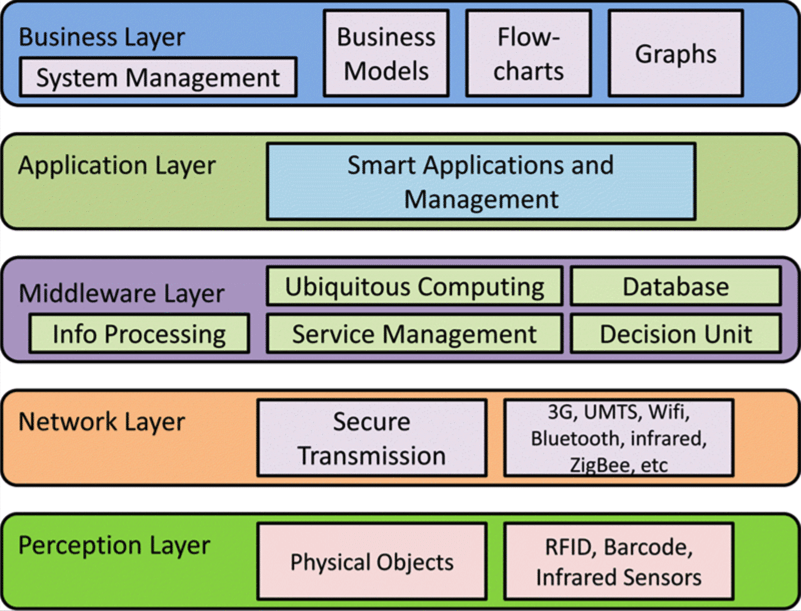
\includegraphics[width=8cm]{archivos/img/teoria/arch_edited.png}
    \caption{Arquitectura básica \glsentryshort{iot}  \cite{carrascal2020diseno}}
    \label{fig:iotBasicArch}
\end{figure}
